\documentclass{article}

\usepackage[%
    left=0.5in,%
    right=0.5in,%
    top=0.5in,%
    bottom=0.5in,%
]{geometry}%
\usepackage{minitoc}
\usepackage{multicol}
\usepackage{graphicx}
\usepackage{fixltx2e}
\usepackage{listings}
\usepackage{color}
\usepackage{hyperref}
    \hypersetup{ colorlinks = true, linkcolor = blue }
\usepackage{blindtext}
\definecolor{lightgray}{gray}{0.9}
\graphicspath{ {./} }

\newcommand{\inlinecode}[2]{\colorbox{lightgray}{\lstinline
[language=#1]$#2$}}
\newcommand{\worddef}[1]{\hyperref[sec:reference]{\textit{#1}}}

\begin{document}

\section{Abstract Data Type: Maps}
\begin{flushleft}
A \textbf{map} models a collection of \textbf{key-value} entries that is searchable \textbf{by the key}. The main operations of a map are for \textbf{searching, inserting, and deleting} items. Multiple entries with the same key are \textbf{not allowed}. (may be allowed in a ‘multi-map’)
\end{flushleft}

\subsection{The Map ADT over K,V}
\begin{flushleft}
Map ADT methods
\begin{itemize}
	\item V get(K k): if the map M has an entry with key k, return its associated value; else, return null
	\item V put(K k, V v): insert entry (k, v) into the map M; if key k is not already in M, then return null; else, return old value associated with k
	\item V remove(K k): if the map M has an entry with key k, remove it from M and return its associated value; else, return null
	\item int size()
	\item boolean isEmpty()
	\item {K} keys(): return an iterable collection of the keys in M
	\item {V} values(): return an iterable collection of the values in M
	\item {<K,V>} entries(): return an iterable collection of the entries in M
\end{itemize}
\end{flushleft}

\subsection{Performance of a List-Based Map}
\begin{itemize}
	\item \texttt{put} would have taken $O(1)$ time if we could just insert the new item at the beginning (or end) of the sequence, but we have to check if the key occurs in the map, so it is $O(n)$.
	\item get and remove take $O(n)$ time since in the worst case (the item is not found) we traverse the entire sequence to look for an item with the given key
\end{itemize}

\section{Hash tables}
\begin{flushleft}
Hash tables are a \textbf{concrete data structure} which is suitable for implementing maps. \textbf{Basic idea}: convert each key into an index into a (big) array. Look-up of keys and insertion and deletion in a hash table usually runs in $O(1)$ time.
\end{flushleft}

\subsection{Hash Functions and Hash Tables}
\begin{flushleft}
A \textbf{hash function} $h()$ maps keys of a given type to integers in a fixed interval $[0, N - 1]$\\
Example: $h(k) = k \; mod \; N$ is a hash function for integer keys. The integer $h(k)$ is called the hash value of key $k$. A hash table for a given key type consists of:
\begin{itemize}
	\item Hash function h
	\item Array (called table) of size N 
\end{itemize}
When implementing a map with a hash table, the goal is to store item (k, v) at index i = h(k)
\end{flushleft}

\subsection{Compression Functions}
\begin{itemize}
	\item Division
	\begin{itemize}
		\item $h2(y) \: = \: y \: mod \: N$
		\item The size $N$ of the hash table is usually chosen to be a \textbf{prime} (hash codes will be spread better)
	\end{itemize}
	\item Multiply, Add and Divide (MAD):
	\begin{itemize}
		\item $h2(y) \: = \: (ay +b) \: mod \: N$
		\item $a$ and $b$ are nonnegative integers such that $a \: mod \: N \: \neq 0$
		\item Otherwise, every integer would map to the same value b
	\end{itemize}
\end{itemize}
\pagebreak

\subsection{Collision Handling}
\begin{flushleft}
Collisions occur when \textbf{different} elements are mapped to the \textbf{same} cell. A lot of the theory and practice of hashing consists of devising better ways to avoid or handle collisions
\end{flushleft}
\begin{itemize}
	\item \textit{Separate Chaining}: let each cell in the table point to (e.g.) a linked list of entries that map there
\end{itemize}

\subsubsection{Map Methods with Separate Chaining used for Collisions}
\begin{flushleft}
Delegate operations to a list-based map at each cell:
\end{flushleft}
\begin{itemize}
	\item \textbf{Algorithm} \texttt{get(k)}:
	\begin{itemize}
	 	\item Output: The value associated with the key $k$ in the map, or \texttt{null} if there is no entry with key equal to k in the map
	 	\item return \inlinecode{C}{A[h(k)].get(k)}
	 	\item {delegate the get to the list-based map at A[h(k)]}
	\end{itemize} 
	\item \textbf{Algorithm} \texttt{put(k,v)}:
	\begin{itemize}
		\item Output:
		\item If there is an existing entry in our map with key equal to k, then we return \textbf{its value} (replacing it with v)
		\item otherwise we return \texttt{null}. \inlinecode{C}{t <- A[h(k)].put(k,v)} 
		\item {delegate the put to the list-based map at A[h(k)]}
	\end{itemize}
	\item \textbf{Algorithm} \texttt{remove(k)}:
	\begin{itemize}
		\item Output:
		\item The (removed) value associated with key $k$ in the map
		\item \texttt{null} if there is no entry with key equal to $k$ in the map
		\item \inlinecode{C}{t <- A[h(k)].remove(k)}
		\item {delegate the remove to the list-based map at A[h(k)]}
	\end{itemize}
\end{itemize}
\begin{flushleft}
Separate chaining is \textbf{simple} and \textbf{fast}, but requires \textbf{additional memory} outside the table.	When memory is critical then try harder to stick with using the existing memory:
\end{flushleft}

\subsection{Open addressing}
\begin{itemize}
	\item Open addressing: the colliding item is placed in a \textbf{different cell} of the table
	\item \textit{Linear probing} handles collisions by placing the colliding item in the \textbf{next} (circularly) available table cell
	\item (variant: cell + c where c is a constant)
	\item Each table cell inspected is referred to as a \textit{probe}
	\item \textbf{Disadvantage}: Colliding items \textbf{lump together}, causing \textbf{future collisions} to cause a longer sequence of probes
\end{itemize}
\begin{flushleft}
\textit{Lazy deletion}: don’t mark the entry as a blank, but as a ‘deleted’ and fix the entries later. E.g. see
\end{flushleft}

\pagebreak

\subsubsection{Search with Linear Probing}
\begin{multicols}{2}
\begin{itemize}
	\item \textbf{Algorithm} \texttt{get(k)}
	\item We start at cell $h(k)$
	\item We probe consecutive locations until one of the following occurs:
	\begin{itemize}
		\item An item with key $k$ is found, or
		\item An \textbf{empty} cell is found, or
		\item $N$ cells have been unsuccessfully probed
	\end{itemize}
\end{itemize}

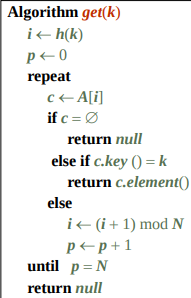
\includegraphics[scale=0.5]{get_open_addressing.png}
\end{multicols}

\subsection{Double Hashing}
\begin{flushleft}
Double hashing uses a \textbf{secondary} hash function $d(k)$ and handles collisions by placing an item in the \textbf{first available cell} of the series
	\[ (h(k) + j d(k)) \: mod \: N \; for  \: j = 0, 1, \: \textrm{...} \: , N - 1 \]
The secondary hash function $d(k)$ \textbf{cannot} have zero values. The table size $N$ must be a \textbf{prime} to allow probing of all the cells (With a prime N, then eventually all table positions will be reached)
\end{flushleft}

\begin{center}
	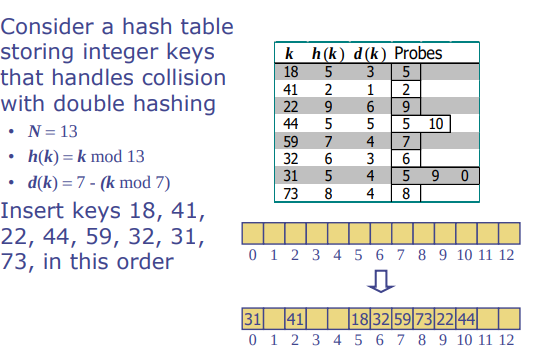
\includegraphics[scale=0.4]{double_hashing.png}
\end{center}

\subsubsection{Performance}
\begin{itemize}
	\item In the worst case, searches, insertions and removals on a hash table take $O(n)$ time (when \textbf{all} the keys inserted into the map \textbf{collide})
	\item The \worddef{load factor} $a \: = \: n/N$ affects the performance of a hash table
	\item In Java, maximal load factor is 0.75 (75\%) – after that, \textit{rehashed}
	\item as for Vector, it is good to \textbf{double} the table size each \textit{rehash} 
	\item The expected running time of all the map ADT operations in a hash table is $O(1)$
	\item In practice, hashing is very \textbf{fast} provided the load factor is not close to \textbf{100\%}
\end{itemize}

\subsection{Rehashing}
\begin{flushleft}
When the table gets too full then \textit{re-hash}: Create a new \textbf{larger} table and \textbf{new hash function}. Need to (eventually) \textbf{transfer} all the entries from the old table to the new one. If do so immediately, then
\begin{itemize}
	\item can amortise the cost over many entries (as for Vector) and so get an average cost of $O(1)$ again
	\item but the worst case might be $O(n)$ when the table is rehashed and this might be bad for a real time system
	\item \textbf{Option}: do not transfer all entries \textbf{in one go} but do \textbf{a few at a time}
	\item Keep \textbf{both} tables until the transfer is complete; but only do \textbf{insertions} into the \textbf{new table}.
\end{itemize}
\end{flushleft}

\subsection{Comparison of HashMap and PQ}
\begin{itemize}
	\item HashMap does not use the ordering of keys
	\item E.g. does not implement \texttt{min()}
	\item In a hash table it would need a scan of all the keys in the table, so $O(n)$ (or worse)
\end{itemize}
\smallskip
\begin{itemize}
	\item PQ does not allow direct access to a key
	\item E.g. there is no easy way to do \texttt{get(k)}
	\item In a (standard) heap we would have to walk through all the entries
\end{itemize}

\pagebreak
\section*{Reference section} \label{sec:reference}
\begin{description}
	\item[load factor] \hfill \\ a measure of how full the hash table is allowed to get before its capacity is automatically increased.
\end{description}
\end{document}
